\section{Q5} 

\subsection{Introduction} \label{sec:Introduction}

Traffic light systems are essential components in urban traffic control, ensuring the safe and orderly flow of 
vehicles and pedestrians. This report focuses on the design and implementation of an automatism for a traffic 
light system using electromagnetic technology, as specified in Question 5 of the lab assignment. The system 
includes three lamps—Red, Yellow, and Green (RYG)—that operate in a timed sequence, and incorporates a sensor 
(S0) to detect pedestrian presence. The objective is to develop a reliable control strategy that adapts the 
light sequence based on pedestrian detection, enhancing both safety and efficiency. The system’s logic is 
structured using Grafcet methodology and simulated in FluidSIM 3.6, allowing for a detailed analysis of the 
control behavior and validation of the functional requirements.

\subsection{Process Schematic and Sensor-Actuator Integration} \label{sec:Process_Schematic_and_Sensor-Actuator_Integration}

\begin{figure}[H]
    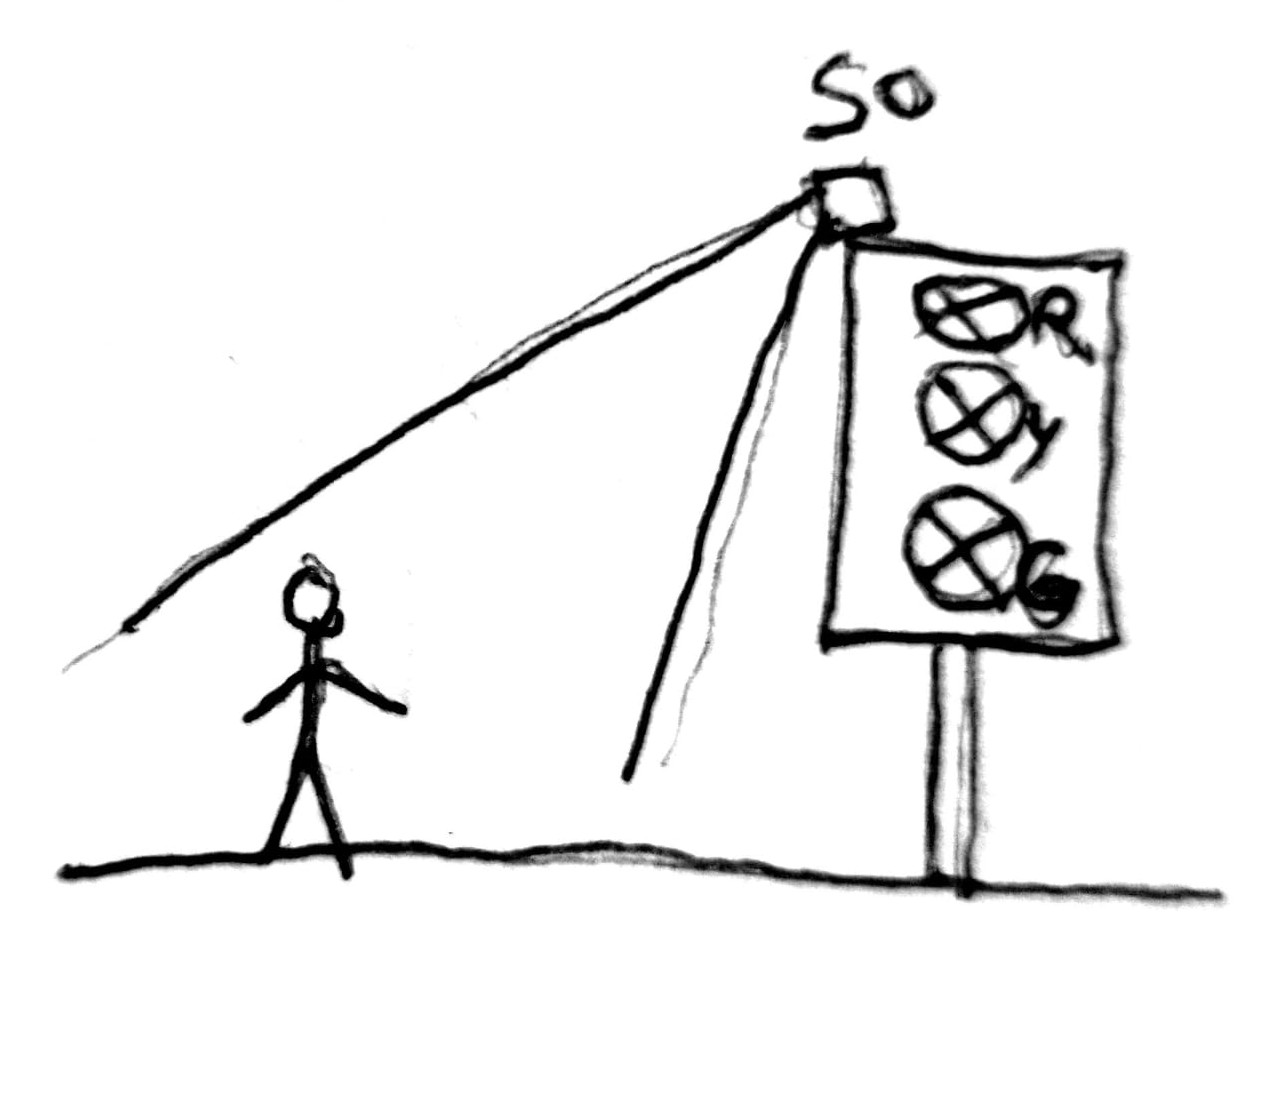
\includegraphics[width=16cm]{Images/Q5/Q5_schem.jpeg}
    \centering
    \caption{Process Schematic for Q5 system}
    \label{fig:Q5_schem}
\end{figure}

\subsection{Control Loop Architecture} \label{sec:Control_Loop_Architecture}

\begin{figure}[H]
    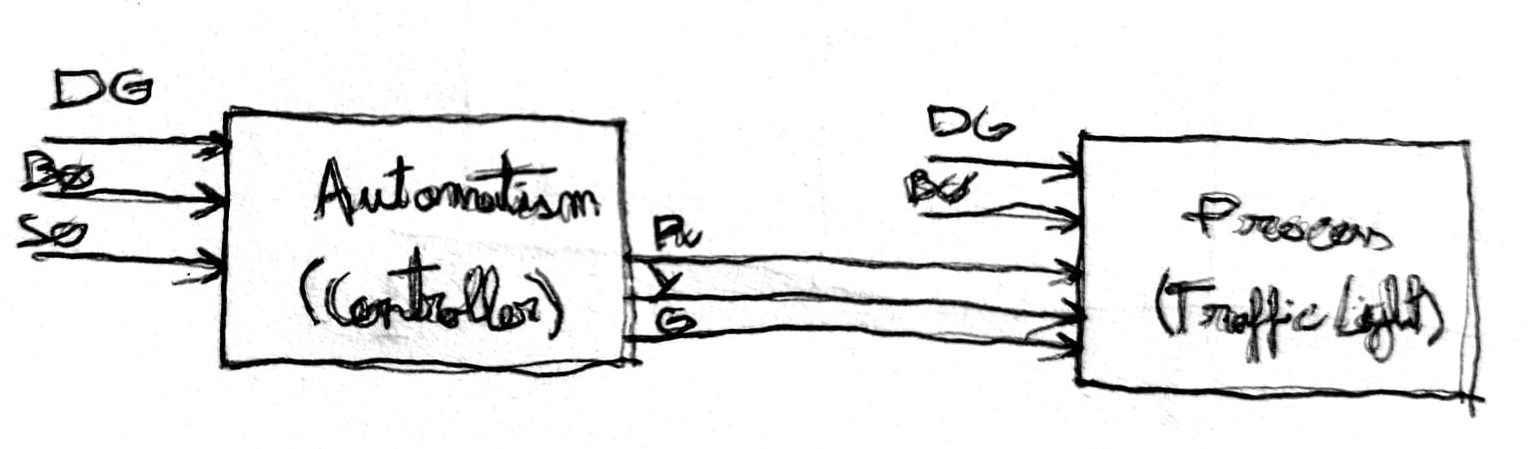
\includegraphics[width=16cm]{Images/Q5/Q5_control.jpeg}
    \centering
    \caption{Control Loop of Q5 system}
    \label{fig:Q5_control}
\end{figure}

\subsection{Grafcet Representation} \label{sec:Grafcet_Representation}

\begin{figure}[H]
    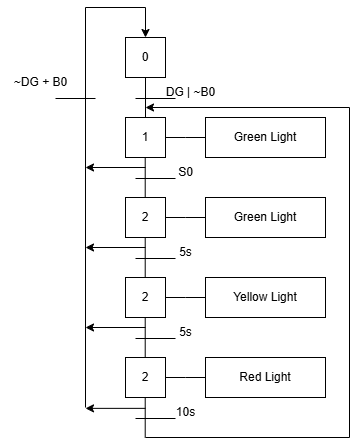
\includegraphics[width=16cm]{Images/Q5/graftset.png}
    \centering
    \caption{Grafset of the street light system}
    \label{fig:grafset}
\end{figure}

\subsection{Simulation and Validation} \label{sec:Simulation_and_Validation}

\begin{figure}[H]
    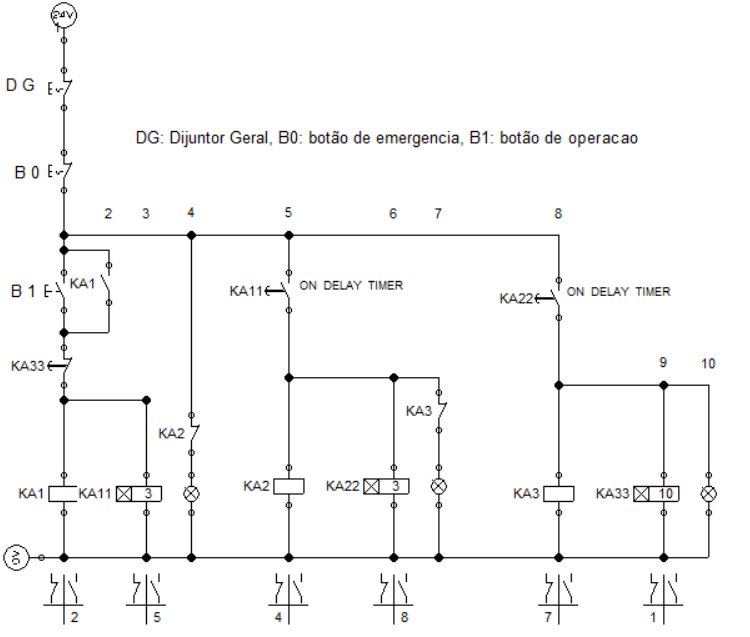
\includegraphics[width=16cm]{Images/Q5/fluidsim.png}
    \centering
    \caption{Fluidsim of the street light system}
    \label{fig:fluidsim}
\end{figure}

\subsection{Conclusion}

This report details the complete development of an electropneumatic control system, from schematic 
design to simulation validation. By integrating various automation components and methodologies, 
the system achieves a robust and efficient control mechanism. The findings highlight the importance 
of precise component selection and control logic design in achieving a functional and reliable 
automated process.